\chapter{Resultados}
\label{chap:resultados}
\label{cap:resultados}

\section{Marcadores eletrocardiográficos}
\label{sec:res-marcadores}

\subsection{Protocolo A: segmentos de 5 minutos}
\label{subsec:res-protocolo-a}

\subsubsection{Comparação univariada}

Dos 44 resumos por paciente, oito apresentaram diferença entre casos e
controles com $p < 0{,}05$ no teste de Mann-Whitney
(\autoref{tab:res-a-univariada}). Com 44 testes, cerca de dois resultados
dessa ordem seriam esperados apenas por acaso. Após a correção de
Benjamini-Hochberg, três permaneceram significativos: o desvio-padrão e a
média da potência HF e o desvio-padrão da frequência cardíaca entre os
segmentos. Os dois desvios-padrão --- da potência HF e da frequência
cardíaca --- sobrevivem também à correção de Bonferroni.

\begin{table}[h!]
	\captionsetup{width=14cm}
	\Caption{\label{tab:res-a-univariada} Marcadores do protocolo A com
		$p < 0{,}05$ na comparação entre casos e controles}
	\IBGEtab{}{
		\begin{tabular}{lrrr}
			\toprule
			Marcador                                 & \multicolumn{1}{c}{Controles} & \multicolumn{1}{c}{Casos} &
			\multicolumn{1}{c}{$p$}                                                                                      \\
			\midrule \midrule
			Potência HF, desvio-padrão               & 0,01                          & 0,02                      & 0,001 \\
			Frequência cardíaca, desvio-padrão (bpm) & 7,84                          & 6,28                      & 0,001 \\
			Potência HF, média                       & 0,01                          & 0,02                      & 0,001 \\
			SD1/SD2, média                           & 0,46                          & 0,56                      & 0,006 \\
			LF/HF, média                             & 2,07                          & 1,50                      & 0,008 \\
			Entropia amostral, média                 & 1,10                          & 0,97                      & 0,013 \\
			Amplitude da derivação Y, média (mV)     & 0,78                          & 0,95                      & 0,030 \\
			Entropia amostral, desvio-padrão         & 0,45                          & 0,39                      & 0,034 \\
			\bottomrule
		\end{tabular}
	}{
		\Fonte{elaborado pelo autor (2026). Valores são medianas em cada grupo.}
	}
\end{table}

A direção das diferenças contraria a leitura clássica da \gls{VFC}. Os
casos apresentaram maior potência HF e maior razão SD1/SD2, isto é, mais
variabilidade de curto prazo, e menor variação da frequência cardíaca ao
longo do registro. Em pacientes com insuficiência cardíaca, variabilidade de
curto prazo elevada pode refletir um ritmo errático, com batimentos
ectópicos e irregularidades não removidos pela correção de artefatos, e não
um tônus vagal preservado. Essa interpretação é coerente com a proporção de
intervalos irregulares, maior nos casos (4,80\,\% contra 2,87\,\%;
$p = 0{,}077$), e com a concentração de valores extremos de SD1 entre os
casos, descrita na \autoref{subsec:met-protocolo-a}.

\subsubsection{Modelos}

A \autoref{tab:res-a-modelos} apresenta o desempenho dos modelos. Os
marcadores, sozinhos, alcançaram \gls{AUC} entre 0,585 e 0,624, com
intervalos de confiança que excluem o acaso por pequena margem. Os melhores
resultados vieram dos modelos que reduzem a dimensão do problema --- a
análise de componentes principais e a floresta aleatória ---, e não das
regressões penalizadas sobre as 44 variáveis. Nenhum modelo baseado apenas
em marcadores alcançou o modelo clínico, de \gls{AUC} 0,661.

\begin{table}[h!]
	\captionsetup{width=15cm}
	\Caption{\label{tab:res-a-modelos} Desempenho dos modelos sobre os
		marcadores do protocolo A}
	\IBGEtab{}{
		\begin{tabular}{lrcrr}
			\toprule
			Modelo                          & \multicolumn{1}{c}{Variáveis} & \gls{AUC} [\glsadd{IC}IC 95\,\%] &
			\multicolumn{1}{c}{Partições}   & \multicolumn{1}{c}{\gls{AP}}                                                      \\
			\midrule \midrule
			Clínicas (referência)           & 6                             & 0,661 [0,577--0,741]  & 0,673 $\pm$ 0,114 & 0,233 \\
			\midrule
			Marcadores, logística L2        & 44                            & 0,589 [0,507--0,671]  & 0,595 $\pm$ 0,066 & 0,180 \\
			Marcadores, logística L1        & 44                            & 0,585 [0,503--0,666]  & 0,588 $\pm$ 0,044 & 0,163 \\
			Marcadores, PCA (4) + logística & 44                            & 0,624 [0,535--0,708]  & 0,623 $\pm$ 0,052 & 0,232 \\
			Marcadores, floresta aleatória  & 44                            & 0,621 [0,537--0,701]  & 0,627 $\pm$ 0,025 & 0,184 \\
			\midrule
			Clínicas + marcadores, L2       & 50                            & 0,672 [0,597--0,745]  & 0,679 $\pm$ 0,099 & 0,201 \\
			Clínicas + marcadores, L1       & 50                            & 0,681 [0,604--0,756]  & 0,690 $\pm$ 0,065 & 0,191 \\
			\bottomrule
		\end{tabular}
	}{
		\Fonte{elaborado pelo autor (2026). Partições: média $\pm$
			desvio-padrão da \gls{AUC} nas cinco partições. \gls{AP} de referência
			(acaso): 0,106.}
	}
\end{table}

Somar os marcadores às variáveis clínicas elevou a \gls{AUC} de 0,661 para
0,672 e 0,681, mas as diferenças não foram distinguíveis de zero:
$+0{,}010$ [$-0{,}056$; $+0{,}086$] com penalização L2 e $+0{,}020$
[$-0{,}047$; $+0{,}095$] com L1.

\subsubsection{Número reduzido de marcadores e otimismo da seleção}

A \autoref{tab:res-a-selecao} compara as duas formas de escolher poucos
marcadores descritas na \autoref{subsec:met-comparacoes-marcadores}. A
partir da análise univariada da coorte inteira, foram escolhidos a média da
potência HF, o desvio-padrão da frequência cardíaca, a média da entropia
amostral e a média da razão SD1/SD2. Esses quatro marcadores alcançaram
\gls{AUC} de 0,627, e os dois primeiros, isoladamente, 0,647. Somados às
variáveis clínicas, produziram os maiores valores deste trabalho, 0,684 e
0,689.

\begin{table}[h!]
	\captionsetup{width=15cm}
	\Caption{\label{tab:res-a-selecao} Efeito da forma de seleção dos
		marcadores no protocolo A}
	\IBGEtab{}{
		\begin{tabular}{llcc}
			\toprule
			Seleção            & Modelo                  & \gls{AUC} [IC 95\,\%] & $\Delta$ sobre clínicas [IC 95\,\%] \\
			\midrule \midrule
			Coorte inteira     & 4 marcadores            & 0,627 [0,541--0,710]  & ---                                 \\
			Coorte inteira     & 2 marcadores            & 0,647 [0,559--0,727]  & ---                                 \\
			Coorte inteira     & clínicas + 4 marcadores & 0,684 [0,601--0,762]  & $+0{,}023$ [$-0{,}027$; $+0{,}078$] \\
			Coorte inteira     & clínicas + 2 marcadores & 0,689 [0,607--0,769]  & $+0{,}027$ [$-0{,}022$; $+0{,}081$] \\
			\midrule
			Dentro da partição & 4 marcadores            & 0,580 [0,497--0,660]  & ---                                 \\
			Dentro da partição & clínicas + 4 marcadores & 0,640 [0,553--0,726]  & $-0{,}021$ [$-0{,}094$; $+0{,}060$] \\
			\bottomrule
		\end{tabular}
	}{
		\Fonte{elaborado pelo autor (2026).}
	}
\end{table}

Quando a seleção foi refeita dentro de cada partição, sem acesso ao
desfecho dos pacientes de teste, a \gls{AUC} dos quatro marcadores caiu para
0,580, com intervalo que inclui o acaso, e a combinação com as variáveis
clínicas ficou abaixo do modelo clínico isolado. A diferença de cerca de
0,05 entre as duas formas de seleção estima o otimismo introduzido por
escolher os marcadores olhando o desfecho de toda a coorte. Os valores
obtidos com seleção dentro da partição são, por isso, os que melhor
representam o desempenho esperado em pacientes novos.

\subsection{Protocolo B: segmentos de 30 segundos}
\label{subsec:res-protocolo-b}

\subsubsection{Pseudorreplicação}

A revisão estatística no nível do segmento foi realizada sobre a primeira
versão da extração, anterior à correção pelos intervalos NN. A
\autoref{tab:res-b-pseudorreplicacao} mostra como a unidade de análise
altera as conclusões. Tratando os 328\,807 segmentos como observações
independentes, 22 dos 24 marcadores diferiram entre casos e controles com
$p < 0{,}05$. No nível do paciente, apenas dois --- a razão SD1/SD2 e a
amplitude da derivação Y --- atingiram esse limiar, e nenhum permaneceu
significativo após as correções para comparações múltiplas.

\begin{table}[h!]
	\captionsetup{width=13cm}
	\Caption{\label{tab:res-b-pseudorreplicacao} Marcadores significativos
		segundo a unidade de análise (24 marcadores)}
	\IBGEtab{}{
		\begin{tabular}{lc}
			\toprule
			Análise                                     & Marcadores com diferença significativa \\
			\midrule \midrule
			Por segmento ($n = 328\,807$), $p < 0{,}05$ & 22                                     \\
			Por paciente ($n = 517$), $p < 0{,}05$      & 2                                      \\
			Por paciente, Benjamini-Hochberg            & 0                                      \\
			Por paciente, Bonferroni                    & 0                                      \\
			\bottomrule
		\end{tabular}
	}{
		\Fonte{elaborado pelo autor (2026).}
	}
\end{table}

O contraste ilustra o problema discutido na
\autoref{subsec:fund-agregacao}. Com centenas de segmentos por paciente,
diferenças mínimas entre os grupos tornam-se estatisticamente
significativas, embora o número real de unidades independentes seja 517.
Foram identificados ainda 26 pares de marcadores redundantes, entre os
quais o RMSSD e o SD1 ($\rho = 0{,}97$), coerentemente com a relação
algébrica entre ambos (\autoref{eq:poincare}).

\subsubsection{Modelos treinados por segmento}

Os modelos treinados diretamente sobre os segmentos, com as probabilidades
agregadas por paciente, permaneceram próximos do acaso
(\autoref{tab:res-b-segmento}). Nenhum intervalo de confiança excluiu 0,5.

\begin{table}[h!]
	\captionsetup{width=13cm}
	\Caption{\label{tab:res-b-segmento} Modelos treinados por segmento de
		30 segundos e avaliados por paciente}
	\IBGEtab{}{
		\begin{tabular}{lcc}
			\toprule
			Modelo                     & \gls{AUC} [IC 95\,\%] & Partições         \\
			\midrule \midrule
			Logística L2               & 0,563 [0,461--0,663]  & 0,569 $\pm$ 0,079 \\
			PCA (6) + logística        & 0,532 [0,442--0,616]  & 0,537 $\pm$ 0,031 \\
			Floresta aleatória         & 0,564 [0,472--0,650]  & 0,576 $\pm$ 0,094 \\
			\textit{Gradient boosting} & 0,549 [0,451--0,636]  & 0,559 $\pm$ 0,114 \\
			\bottomrule
		\end{tabular}
	}{
		\Fonte{elaborado pelo autor (2026).}
	}
\end{table}

\subsubsection{Modelos sobre os resumos por paciente}

A \autoref{tab:res-b-paciente} apresenta as doze configurações avaliadas
sobre os resumos por paciente da extração corrigida. Onze delas tiveram
intervalo de confiança que inclui 0,5. A única exceção, a análise de
componentes principais sobre o conjunto B, com \gls{AUC} de 0,619
[0,537--0,700], é a melhor de doze tentativas e deve ser interpretada com a
correspondente cautela. A versão da extração anterior à correção NN produziu
o mesmo quadro, com o melhor resultado em 0,583 [0,483--0,674].

\begin{table}[h!]
	\captionsetup{width=15cm}
	\Caption{\label{tab:res-b-paciente} Modelos sobre os resumos por paciente
		dos segmentos de 30 segundos (extração corrigida)}
	\IBGEtab{}{
		\begin{tabular}{lrcccc}
			\toprule
			Conjunto                   & \multicolumn{1}{c}{Variáveis} & Logística L2 & Logística L1 &
			PCA (4) + logística        & Floresta aleatória                                                          \\
			\midrule \midrule
			A (mediana)                & 32                            & 0,552        & 0,550        & 0,563 & 0,532 \\
			B (A + dispersão e fração) & 64                            & 0,540        & 0,548        & 0,619 & 0,562 \\
			C (todos os resumos)       & 122                           & 0,545        & 0,550        & 0,548 & 0,582 \\
			\bottomrule
		\end{tabular}
	}{
		\Fonte{elaborado pelo autor (2026). Valores de \gls{AUC} das predições
			fora da partição.}
	}
\end{table}

Na comparação univariada dos 122 resumos, sete apresentaram $p < 0{,}05$,
número próximo do esperado por acaso, e nenhum permaneceu significativo após
a correção de Benjamini-Hochberg. Os menores valores-$p$ concentraram-se,
porém, em um padrão consistente: medidas de dispersão ao longo do registro
foram menores nos casos, como o intervalo interquartil do QT (35 contra
45\,ms; $p < 0{,}001$; $q = 0{,}083$) e o da frequência cardíaca (9,9
contra 11,5\,bpm; $p = 0{,}004$). O mesmo padrão apareceu no protocolo A,
no qual o desvio-padrão da frequência cardíaca entre os segmentos foi um dos
três marcadores que resistiram à correção para comparações múltiplas.

\subsection{Síntese}
\label{subsec:res-marcadores-sintese}

A \autoref{tab:res-marcadores-sintese} reúne os principais resultados. Os
marcadores extraídos do \gls{ECG} contêm informação sobre o desfecho, mas
essa informação é fraca: nos melhores casos, a \gls{AUC} situou-se entre 0,60
e 0,65, e cai para perto do acaso quando a escolha dos marcadores é feita
sem acesso ao desfecho dos pacientes de teste. Em nenhuma configuração os
marcadores superaram as seis variáveis clínicas, nem acrescentaram a elas
um ganho distinguível de zero. O sinal mais consistente entre os dois
protocolos foi a menor variação da frequência cardíaca ao longo do registro
entre os pacientes que sofreram \gls{MSC}.

\begin{table}[h!]
	\captionsetup{width=15cm}
	\Caption{\label{tab:res-marcadores-sintese} Síntese dos resultados com
		marcadores eletrocardiográficos}
	\IBGEtab{}{
		\begin{tabular}{lc}
			\toprule
			Modelo                                                   & \gls{AUC} [IC 95\,\%] \\
			\midrule \midrule
			Clínicas (referência)                                    & 0,661 [0,577--0,741]  \\
			Protocolo A, PCA (4) + logística                         & 0,624 [0,535--0,708]  \\
			Protocolo A, 4 marcadores com seleção dentro da partição & 0,580 [0,497--0,660]  \\
			Protocolo A, clínicas + marcadores (L1)                  & 0,681 [0,604--0,756]  \\
			Protocolo B, por segmento (melhor de quatro)             & 0,564 [0,472--0,650]  \\
			Protocolo B, por paciente (melhor de doze)               & 0,619 [0,537--0,700]  \\
			\bottomrule
		\end{tabular}
	}{
		\Fonte{elaborado pelo autor (2026).}
	}
\end{table}

\citeonline{swee2026multimodal} relatam, na mesma base, \gls{AUC} de
0,682 $\pm$ 0,030 com um modelo apenas de \gls{ECG} sobre marcadores de
segmentos de 30~segundos. A comparação direta é limitada: aquele trabalho
utilizou 746 pacientes, sem restrição ao ritmo sinusal e com critérios de
exclusão distintos, e reporta a média entre partições, enquanto a métrica
principal deste trabalho é a \gls{AUC} das predições agrupadas. Na mesma
métrica, a média entre partições, os modelos por segmento deste trabalho
alcançaram entre 0,537 e 0,576.


% ==============================================================================
% RESULTADOS — Redes neurais sobre o sinal de Holter
% Fontes: logs classificacao_*.log, optuna_*.log (rodada final em 5 partições).
% Todos os valores verificados nos logs. Coorte: 517 pacientes, 55 casos.
% CNN média de 2 min: execução refeita em 16/10/2026 (a primeira falhou por
% checkpoint compartilhado com a CNN simples).
% Configuração das ResNets (20 épocas, paciência 10, 250 janelas de treino e
% 100 de avaliação por paciente) difere da das CNNs (30 épocas, paciência 15,
% 350 e 200 janelas) — declarado no texto.
% ==============================================================================

\section{Redes neurais sobre o sinal de Holter}
\label{sec:res-redes}

Esta seção apresenta o desempenho das redes neurais treinadas diretamente
sobre o sinal das três derivações do Holter. Todas foram avaliadas pelo mesmo
protocolo: cinco partições estratificadas sobre os 517 pacientes, com 309 ou
310 pacientes de treinamento, 104 de validação interna e 103 ou 104 de teste
em cada partição. O valor principal é a \gls{AUC} fora da partição,
calculada sobre as predições dos 517 pacientes, cada um predito pelo modelo
que não o viu no treinamento, com intervalo de confiança de 95\,\% obtido por
\textit{bootstrap}. A média e o desvio-padrão da \gls{AUC} entre as cinco
partições são informados ao lado, como medida da instabilidade do resultado.

\subsection{Redes convolucionais: capacidade e duração da janela}
\label{subsec:res-cnn-capacidade}

A \autoref{tab:res-cnn-capacidade} apresenta as redes convolucionais do
desenho da \autoref{subsec:met-cnn-experimentos}, que varia a capacidade da
rede e a duração da janela de entrada.

\begin{table}[h!]
	\captionsetup{width=15cm}
	\Caption{\label{tab:res-cnn-capacidade} Desempenho das redes
		convolucionais segundo a capacidade e a duração da janela}
	\IBGEtab{}{
		\begin{tabular}{llrcc}
			\toprule
			Rede                & Janela                                 & \multicolumn{1}{c}{Parâmetros} &
			\gls{AUC} partições & \gls{AUC} fora da partição [IC 95\,\%]                                                                             \\
			\midrule \midrule
			Mínima              & 2 min                                  & 14\,425                        & 0,543 $\pm$ 0,059 & 0,523 [0,440--0,612] \\
			Simples             & 2 min                                  & 109\,361                       & 0,500 $\pm$ 0,067 & 0,486 [0,402--0,578] \\
			Média               & 2 min                                  & 418\,145                       & 0,494 $\pm$ 0,119 & 0,485 [0,400--0,574] \\
			\midrule
			Mínima              & 10 s                                   & 14\,425                        & 0,589 $\pm$ 0,090 & 0,554 [0,467--0,634] \\
			Simples             & 10 s                                   & 109\,361                       & 0,509 $\pm$ 0,051 & 0,491 [0,411--0,578] \\
			Média               & 10 s                                   & 418\,145                       & 0,495 $\pm$ 0,118 & 0,485 [0,406--0,569] \\
			\bottomrule
		\end{tabular}
	}{
		\Fonte{elaborado pelo autor (2026).}
	}
\end{table}

Nenhuma configuração se distinguiu do acaso: todos os intervalos de
confiança incluem 0,5. A rede mínima obteve os maiores valores nas duas
durações de janela. Nas duas durações, o desempenho caiu à medida que a
capacidade aumentou: 0,523, 0,486 e 0,485 com a janela de 2~minutos e
0,554, 0,491 e 0,485 com a de 10~segundos. A diferença entre a rede
mínima e a média, no entanto, é menor que a largura de qualquer um dos
intervalos e não permite afirmar uma relação entre capacidade e desempenho.
O mesmo vale para a duração da janela: a rede mínima obteve 0,523 com
2~minutos e 0,554 com 10~segundos, valores compatíveis entre si.

\subsection{Redes residuais: largura da ResNet-18}
\label{subsec:res-resnet18-largura}

As redes residuais foram treinadas com uma configuração anterior à das redes
convolucionais da seção precedente: 20 épocas no máximo, paciência de
10 épocas, 250 janelas de treinamento e 100 de avaliação por paciente. A
\autoref{tab:res-resnet18-largura} compara três larguras da ResNet-18, que
mantêm os quatro estágios de dois blocos e variam o número de canais.

\begin{table}[h!]
	\captionsetup{width=15cm}
	\Caption{\label{tab:res-resnet18-largura} Desempenho da ResNet-18 em três
		larguras}
	\IBGEtab{}{
		\begin{tabular}{llrcc}
			\toprule
			Rede                & Janela                                 & \multicolumn{1}{c}{Parâmetros} &
			\gls{AUC} partições & \gls{AUC} fora da partição [IC 95\,\%]                                                                             \\
			\midrule \midrule
			ResNet-18 mínima    & 5,12 s                                 & 78\,169                        & 0,569 $\pm$ 0,067 & 0,562 [0,475--0,642] \\
			ResNet-18 reduzida  & 2 min                                  & 1\,029\,985                    & 0,516 $\pm$ 0,102 & 0,504 [0,420--0,588] \\
			ResNet-18 completa  & 2 min                                  & 3\,976\,385                    & 0,528 $\pm$ 0,088 & 0,508 [0,431--0,588] \\
			ResNet-18 completa  & 5,12 s                                 & 3\,976\,385                    & 0,500 $\pm$ 0,080 & 0,492 [0,411--0,577] \\
			\bottomrule
		\end{tabular}
	}{
		\Fonte{elaborado pelo autor (2026).}
	}
\end{table}

A versão mínima, com 78~mil parâmetros (253 por paciente de treinamento),
obteve o maior valor entre as redes residuais (0,562), e as versões reduzida
e completa ficaram em torno de 0,50. Assim como nas redes convolucionais, a
redução da largura retardou a memorização dos pacientes de treinamento, mas
o intervalo de confiança da versão mínima ainda inclui 0,5. A ResNet-18
completa obteve resultados equivalentes com janelas de 2~minutos e de
5,12~segundos.

\subsection{Redes residuais: profundidade (ResNet-18, ResNet-34 e ResNet-50)}
\label{subsec:res-resnet-profundidade}

A \autoref{tab:res-resnet-profundidade} compara redes residuais de 18, 34 e
50 camadas com a mesma largura e a mesma janela de 2~minutos. A ResNet-34
empilha mais blocos básicos em cada estágio, e a ResNet-50 substitui o bloco
básico pelo bloco de gargalo (\autoref{sec:fund-resnet}).

\begin{table}[h!]
	\captionsetup{width=15cm}
	\Caption{\label{tab:res-resnet-profundidade} Desempenho das redes
		residuais segundo a profundidade}
	\IBGEtab{}{
		\begin{tabular}{lrrcc}
			\toprule
			Rede                             & \multicolumn{1}{c}{Parâmetros}         &
			\multicolumn{1}{c}{Por paciente} &
			\gls{AUC} partições              & \gls{AUC} fora da partição [IC 95\,\%]                                                      \\
			\midrule \midrule
			ResNet-18                        & 3\,976\,385                            & 12\,869 & 0,528 $\pm$ 0,088 & 0,508 [0,431--0,588] \\
			ResNet-34                        & 7\,350\,721                            & 23\,789 & 0,540 $\pm$ 0,039 & 0,514 [0,429--0,601] \\
			ResNet-50                        & 16\,479\,937                           & 53\,333 & 0,569 $\pm$ 0,098 & 0,536 [0,448--0,618] \\
			\bottomrule
		\end{tabular}
	}{
		\Fonte{elaborado pelo autor (2026). Parâmetros por paciente de
			treinamento (309 pacientes).}
	}
\end{table}

Quadruplicar o número de parâmetros, da ResNet-18 para a ResNet-50, não
alterou o desempenho: os três valores ficaram entre 0,51 e 0,54, com
intervalos amplamente sobrepostos e todos incluindo 0,5. A ResNet-50, com
mais de 53~mil parâmetros por paciente de treinamento, memorizou o conjunto
de treinamento já nas primeiras épocas, como as demais, e não extraiu do
sinal informação adicional.

\subsection{ResNet-18 com mecanismo de atenção}
\label{subsec:res-resnet-atencao}

Na rede com atenção, as características extraídas pela ResNet-18 ao
longo da janela são relacionadas entre si por um codificador
\textit{Transformer} antes do agrupamento (\autoref{sec:fund-atencao}),
totalizando 1\,491\,553 parâmetros. A \gls{AUC} fora da partição foi de
0,493 [0,419--0,577], com média entre partições de 0,512 $\pm$ 0,041. A
modelagem explícita das relações temporais dentro da janela de 2~minutos,
portanto, não acrescentou capacidade discriminativa à ResNet-18.

\subsection{Busca de hiperparâmetros}
\label{subsec:res-redes-optuna}

Para verificar se o desempenho dependia de uma escolha inadequada de
hiperparâmetros, uma rede convolucional e uma rede residual foram
configuradas por busca bayesiana com o \textit{Optuna}
(\autoref{tab:res-redes-optuna}). Foram feitas 25 tentativas para cada
família, variando largura, profundidade, tipo de agrupamento, taxa de
aprendizado, decaimento de pesos, descarte e duração da janela. A busca
maximizou a \gls{AUC} média da validação interna em três partições, sem
acesso aos conjuntos de teste, e a configuração escolhida foi avaliada nas
cinco partições do protocolo.

\begin{table}[h!]
	\captionsetup{width=15cm}
	\Caption{\label{tab:res-redes-optuna} Desempenho das redes configuradas
		por busca de hiperparâmetros}
	\IBGEtab{}{
		\begin{tabular}{llrcc}
			\toprule
			Rede                & Janela                                 & \multicolumn{1}{c}{Parâmetros} &
			\gls{AUC} partições & \gls{AUC} fora da partição [IC 95\,\%]                                                                             \\
			\midrule \midrule
			Convolucional$^{a}$ & 1 min                                  & 473\,417                       & 0,574 $\pm$ 0,112 & 0,556 [0,464--0,647] \\
			Residual$^{b}$      & 1 min                                  & 1\,818\,049                    & 0,510 $\pm$ 0,079 & 0,496 [0,411--0,584] \\
			\bottomrule
		\end{tabular}
	}{
		\Fonte{elaborado pelo autor (2026). $^{a}$Quatro blocos com 24, 48, 96 e
			96 canais, núcleo de 31 amostras e agrupamento por média.
			$^{b}$ResNet com quatro estágios de um bloco, 64 canais iniciais e
			agrupamento por máximo.}
	}
\end{table}

A busca não superou as configurações escolhidas manualmente. A rede
convolucional encontrada obteve 0,556, o mesmo valor da rede convolucional
mínima sem busca (0,554), e a rede residual obteve 0,496. Como os
hiperparâmetros foram escolhidos pela validação interna, e não em uma
validação cruzada aninhada, mesmo esses valores carregam algum otimismo
residual.

\subsection{Comportamento durante o treinamento}
\label{subsec:res-redes-treino}

Os registros de treinamento mostram o mesmo padrão em todas as arquiteturas.
A perda de treinamento cai rapidamente --- na ResNet-18, de cerca de 0,65
para menos de 0,02 em dez épocas ---, enquanto a perda de validação sobe
desde a segunda ou terceira época, de cerca de 1,5 para valores entre 4 e 8.
A rede memoriza os pacientes de treinamento em vez de aprender um padrão que
se transfira para pacientes novos. As redes de menor capacidade retardam esse
processo: na rede convolucional mínima, a perda de treinamento ainda estava
em torno de 0,55 ao final das 30 épocas, e é nela que se observaram os
maiores valores de \gls{AUC}, ainda que não significativos.

A \gls{AUC} de validação mostrou-se um indicador pouco confiável do
desempenho no teste. Na quarta partição da rede convolucional média, por
exemplo, a validação interna atingiu \gls{AUC} de 0,64, e o teste, 0,30; na
terceira partição da ResNet-50, a validação chegou a 0,75 e o teste ficou em
0,49. Com 11 casos na validação interna, a \gls{AUC} de validação oscila o
suficiente entre épocas para que a escolha do melhor modelo seja, em boa
parte, determinada pelo acaso.

\subsection{Variabilidade entre execuções}
\label{subsec:res-redes-reprodutibilidade}

A ResNet-18 mínima, com janela de 5,12~segundos, foi treinada duas vezes
sobre as mesmas partições, alterando-se apenas o tamanho do lote (2\,000 e
1\,000 janelas) e o número de janelas sorteadas por paciente (500 e 850). A
\gls{AUC} fora da partição passou de 0,562 [0,475--0,642] para 0,480
[0,403--0,557]. Essa diferença de 0,08 entre duas execuções da mesma
arquitetura é maior que a diferença entre a rede de melhor e a de pior
desempenho entre as redes convolucionais e residuais avaliadas.
O desvio-padrão da \gls{AUC} entre partições, entre 0,04 e 0,12, aponta na
mesma direção. A ordenação das arquiteturas, portanto, não deve ser
interpretada como evidência de superioridade de uma sobre as outras.

\subsection{Fusão da ResNet-18 com variáveis clínicas}
\label{subsec:res-redes-fusao}

A rede de fusão combina o extrator da ResNet-18 com um ramo que recebe seis
variáveis clínicas --- idade, sexo, classe funcional da \gls{NYHA}, ondas Q, taquicardia ventricular não sustentada e taquiarritmia supraventricular paroxística ---,
totalizando 3\,987\,041 parâmetros, dos quais 10\,656
pertencem ao ramo clínico. A \autoref{tab:res-fusao} compara as três
estratégias de treinamento descritas na \autoref{subsec:met-fusao}.

\begin{table}[h!]
	\captionsetup{width=15cm}
	\Caption{\label{tab:res-fusao} Desempenho da rede de fusão segundo a
		estratégia de treinamento do extrator de sinal}
	\IBGEtab{}{
		\begin{tabular}{llcc}
			\toprule
			Estratégia                & Janela & \gls{AUC} partições &
			\gls{AUC} fora da partição [IC 95\,\%]                                          \\
			\midrule \midrule
			Treinamento conjunto      & 2 min  & 0,534 $\pm$ 0,090   & 0,516 [0,433--0,603] \\
			Taxa reduzida no extrator & 2 min  & 0,578 $\pm$ 0,046   & 0,579 [0,492--0,669] \\
			Extrator congelado$^{a}$  & 2 min  & 0,572 $\pm$ 0,043   & 0,577 [0,491--0,659] \\
			Treinamento conjunto      & 10 s   & 0,492 $\pm$ 0,105   & 0,491 [0,409--0,576] \\
			\bottomrule
		\end{tabular}
	}{
		\Fonte{elaborado pelo autor (2026). $^{a}$142\,241 parâmetros
			treináveis; o extrator de sinal permanece com os pesos iniciais.}
	}
\end{table}

O resultado é informativo justamente pelo contraste entre as estratégias.
Quando o extrator de sinal é congelado, a rede ajusta apenas o ramo clínico e
o classificador, e a \gls{AUC} chega a 0,577. Quando o extrator aprende com
taxa reduzida, o resultado é praticamente o mesmo (0,579). Quando o extrator
é treinado livremente, junto com o restante da rede, a \gls{AUC} cai para
0,516. Ou seja, o desempenho da rede de fusão vem das variáveis
clínicas, e o sinal, quando treinado, introduz variabilidade que prejudica a
discriminação em vez de acrescentar informação. Para referência, o modelo
logístico sobre as variáveis clínicas, sem nenhuma informação do sinal,
obteve 0,661 [0,577--0,741] (\autoref{tab:res-a-modelos}).

\subsection{Análise de sensibilidade: ResNet-18 sem restrição ao ritmo sinusal}
\label{subsec:res-redes-ritmo}

Para verificar se o pipeline é capaz de extrair do sinal alguma informação
associada ao desfecho, a ResNet-18 foi treinada também sobre a coorte sem o
critério de ritmo sinusal, com 703 pacientes e 85 casos. Nessa coorte, a
\gls{AUC} fora da partição foi de 0,575 [0,511--0,642], o único intervalo
entre as redes que exclui 0,5 (média entre partições de 0,601 $\pm$ 0,049).
Esse ganho não pode ser atribuído a um marcador de morte súbita: a coorte
ampliada inclui pacientes em fibrilação atrial, um ritmo facilmente
reconhecível no sinal e associado a pior prognóstico. A rede tem, portanto,
um atalho para discriminar os grupos que não existe na coorte restrita ao
ritmo sinusal. O resultado mostra que o pipeline aprende quando há um padrão
reconhecível no sinal e justifica a restrição adotada na
\autoref{sec:intro-dados}, que remove essa fonte de confundimento.

\subsection{Métricas dependentes de limiar}
\label{subsec:res-redes-limiar}

A \autoref{tab:res-redes-limiar} reúne, para todas as redes do protocolo
principal, as métricas calculadas sobre as predições fora da partição após a
aplicação do limiar de decisão escolhido na validação interna.

\begin{table}[h!]
	\captionsetup{width=16cm}
	\Caption{\label{tab:res-redes-limiar} Métricas dependentes de limiar das
	redes neurais, calculadas sobre as predições fora da partição dos 517
	pacientes}
	\IBGEtab{}{
		\footnotesize
		\setlength{\tabcolsep}{4pt}
		\begin{tabular}{llcccccccc}
			\toprule
			Rede & Janela & \gls{AUC} & \gls{AP} & Sens. & Espec. & \gls{VPP} & \gls{VPN} & F1 & Acurácia \\
			\midrule \midrule
			CNN mínima & 2 min & 0,523 & 0,139 & 0,582 & 0,448 & 0,111 & 0,900 & 0,187 & 0,462 \\
			CNN simples & 2 min & 0,486 & 0,121 & 0,364 & 0,645 & 0,109 & 0,895 & 0,167 & 0,615 \\
			CNN média & 2 min & 0,485 & 0,126 & 0,309 & 0,688 & 0,106 & 0,893 & 0,157 & 0,648 \\
			CNN mínima & 10 s & 0,554 & 0,132 & 0,691 & 0,346 & 0,112 & 0,904 & 0,192 & 0,383 \\
			CNN simples & 10 s & 0,491 & 0,119 & 0,400 & 0,530 & 0,092 & 0,881 & 0,150 & 0,516 \\
			CNN média & 10 s & 0,485 & 0,110 & 0,455 & 0,485 & 0,095 & 0,882 & 0,157 & 0,482 \\
			\midrule
			ResNet-18 mínima & 5,12 s & 0,562 & 0,160 & 0,455 & 0,654 & 0,135 & 0,910 & 0,208 & 0,632 \\
			ResNet-18 reduzida & 2 min & 0,504 & 0,117 & 0,582 & 0,437 & 0,110 & 0,898 & 0,184 & 0,453 \\
			ResNet-18 completa & 2 min & 0,508 & 0,121 & 0,455 & 0,461 & 0,091 & 0,877 & 0,152 & 0,460 \\
			ResNet-18 completa & 5,12 s & 0,492 & 0,129 & 0,582 & 0,442 & 0,110 & 0,899 & 0,186 & 0,456 \\
			ResNet-34 & 2 min & 0,514 & 0,122 & 0,509 & 0,517 & 0,112 & 0,898 & 0,183 & 0,516 \\
			ResNet-50 & 2 min & 0,536 & 0,137 & 0,455 & 0,511 & 0,100 & 0,887 & 0,163 & 0,505 \\
			ResNet-18 + Transformer & 2 min & 0,493 & 0,134 & 0,291 & 0,703 & 0,105 & 0,893 & 0,154 & 0,660 \\
			\midrule
			Convolucional, busca & 1 min & 0,556 & 0,189 & 0,509 & 0,552 & 0,119 & 0,904 & 0,193 & 0,547 \\
			Residual, busca & 1 min & 0,496 & 0,122 & 0,455 & 0,565 & 0,111 & 0,897 & 0,178 & 0,553 \\
			\midrule
			Fusão, treino conjunto & 2 min & 0,516 & 0,141 & 0,418 & 0,548 & 0,099 & 0,888 & 0,160 & 0,534 \\
			Fusão, taxa reduzida & 2 min & 0,579 & 0,180 & 0,455 & 0,673 & 0,142 & 0,912 & 0,216 & 0,650 \\
			Fusão, extrator congelado & 2 min & 0,577 & 0,146 & 0,727 & 0,424 & 0,131 & 0,929 & 0,222 & 0,456 \\
			Fusão, treino conjunto & 10 s & 0,491 & 0,113 & 0,400 & 0,569 & 0,100 & 0,889 & 0,159 & 0,551 \\
			\bottomrule
		\end{tabular}
	}{
	\Fonte{elaborado pelo autor (2026). Limiar de decisão escolhido pelo índice
	de Youden na validação interna de cada partição. Referência sob
	classificação aleatória: \gls{AP} e \gls{VPP} iguais à prevalência
	(0,106); \gls{VPN} igual a 0,894.}
}
\end{table}


As métricas dependentes de limiar confirmam o quadro da \gls{AUC}. O
\gls{VPP} ficou entre 0,09 e 0,14 em todas as redes, próximo da prevalência
de 0,106, ou seja, entre os pacientes classificados como de alto risco a
proporção de casos foi praticamente a mesma da coorte. O \gls{VPN}, entre
0,88 e 0,93, também se manteve próximo do valor de 0,894 que se obteria
classificando todos os pacientes como controles. A sensibilidade e a
especificidade variaram em sentidos opostos entre as redes --- de 0,29 a
0,73 e de 0,35 a 0,70, respectivamente ---, o que reflete apenas a posição
do limiar, e não uma capacidade de separação: as redes de maior
sensibilidade são as de menor especificidade. A acurácia, entre 0,38 e 0,66,
fica sempre abaixo dos 0,894 obtidos pela classificação trivial de todos os
pacientes como controles, o que ilustra por que ela não é adequada com
classes desbalanceadas. A rede de fusão com extrator congelado obteve a
maior sensibilidade (0,727) com \gls{VPN} de 0,929, mas à custa de
especificidade de 0,424.

A \autoref{tab:res-redes-confusao} apresenta as matrizes de confusão que
originam essas métricas. Em todas as redes, o número de controles
classificados como de alto risco (FP) supera em várias vezes o de casos
corretamente identificados (VP): para cada morte súbita detectada, entre
seis e dez sobreviventes foram classificados como de alto risco.

\begin{table}[h!]
	\captionsetup{width=14cm}
	\Caption{\label{tab:res-redes-confusao} Limiar de decisão e matriz de
	confusão agregada das redes neurais sobre os 517 pacientes}
	\IBGEtab{}{
		\footnotesize
		\begin{tabular}{llccccc}
			\toprule
			Rede & Janela & Limiar & VP & FN & FP & VN \\
			\midrule \midrule
			CNN mínima & 2 min & 0,460 & 32 & 23 & 255 & 207 \\
			CNN simples & 2 min & 0,409 & 20 & 35 & 164 & 298 \\
			CNN média & 2 min & 0,357 & 17 & 38 & 144 & 318 \\
			CNN mínima & 10 s & 0,348 & 38 & 17 & 302 & 160 \\
			CNN simples & 10 s & 0,246 & 22 & 33 & 217 & 245 \\
			CNN média & 10 s & 0,268 & 25 & 30 & 238 & 224 \\
			\midrule
			ResNet-18 mínima & 5,12 s & 0,489 & 25 & 30 & 160 & 302 \\
			ResNet-18 reduzida & 2 min & 0,092 & 32 & 23 & 260 & 202 \\
			ResNet-18 completa & 2 min & 0,058 & 25 & 30 & 249 & 213 \\
			ResNet-18 completa & 5,12 s & 0,186 & 32 & 23 & 258 & 204 \\
			ResNet-34 & 2 min & 0,154 & 28 & 27 & 223 & 239 \\
			ResNet-50 & 2 min & 0,032 & 25 & 30 & 226 & 236 \\
			ResNet-18 + Transformer & 2 min & 0,040 & 16 & 39 & 137 & 325 \\
			\midrule
			Convolucional, busca & 1 min & -- & 28 & 27 & 207 & 255 \\
			Residual, busca & 1 min & -- & 25 & 30 & 201 & 261 \\
			\midrule
			Fusão, treino conjunto & 2 min & 0,062 & 23 & 32 & 209 & 253 \\
			Fusão, taxa reduzida & 2 min & 0,489 & 25 & 30 & 151 & 311 \\
			Fusão, extrator congelado & 2 min & 0,447 & 40 & 15 & 266 & 196 \\
			Fusão, treino conjunto & 10 s & 0,026 & 22 & 33 & 199 & 263 \\
			\bottomrule
		\end{tabular}
	}{
	\Fonte{elaborado pelo autor (2026). VP: casos classificados como de alto
	risco; FN: casos classificados como de baixo risco; FP: controles
	classificados como de alto risco; VN: controles classificados como de
	baixo risco. Total de 55 casos e 462 controles. Limiar: mediana dos
	limiares de Youden das cinco partições; não registrado nas redes
	configuradas por busca.}
}
\end{table}


\subsection{Síntese}
\label{subsec:res-redes-sintese}

Em 19 configurações avaliadas no protocolo principal, nenhuma rede treinada
sobre o sinal do Holter discriminou casos e controles de forma distinguível
do acaso. Os valores de \gls{AUC} fora da partição ficaram entre 0,48 e
0,56, sem relação com a capacidade da rede, com a duração da janela ou com a
presença de mecanismos de atenção, e a variação entre execuções da mesma rede
foi da mesma ordem que a variação entre arquiteturas. Na rede de fusão, o
sinal não acrescentou informação às variáveis clínicas. Esses resultados são
coerentes com o tamanho da amostra: com 33 casos de treinamento por
partição, mesmo a menor das redes tem centenas de parâmetros por caso, e a
evidência disponível não sustenta a existência de um padrão no sinal de
Holter, em ritmo sinusal, que antecipe a morte súbita nesta coorte.

% ==============================================================================
% RESULTADOS — ECG de repouso de alta resolução com arquitetura CNN-LSTM
% Fonte: cnnlstm_res.log (5 partições)
%
% ⚠️ A coorte desta seção (367 pacientes, 41 eventos) difere da utilizada nas
%    demais (517 pacientes, 55 eventos). O texto registra a limitação que
%    isso impõe à comparação.
% ==============================================================================

\section{Representações aprendidas com rótulos substitutos}
\label{sec:res-substitutos}

Esta seção apresenta os modelos descritos na \autoref{sec:met-substitutos},
avaliados nas mesmas cinco partições. A \autoref{fig:res-substitutos} reúne
as \gls{AUC} fora da partição dos principais modelos, e a
\autoref{tab:res-substitutos}, as métricas dependentes de limiar.

\begin{figure}[h!]
	\captionsetup{width=16cm}
	\Caption{\label{fig:res-substitutos} \gls{AUC} fora da partição, com
		intervalo de confiança de 95\,\%, dos modelos sobre o sinal sem rótulos
		clínicos, orientados por conhecimento clínico, das variáveis do estudo
		MUSIC e de suas combinações}
	\UFCfig{}{
		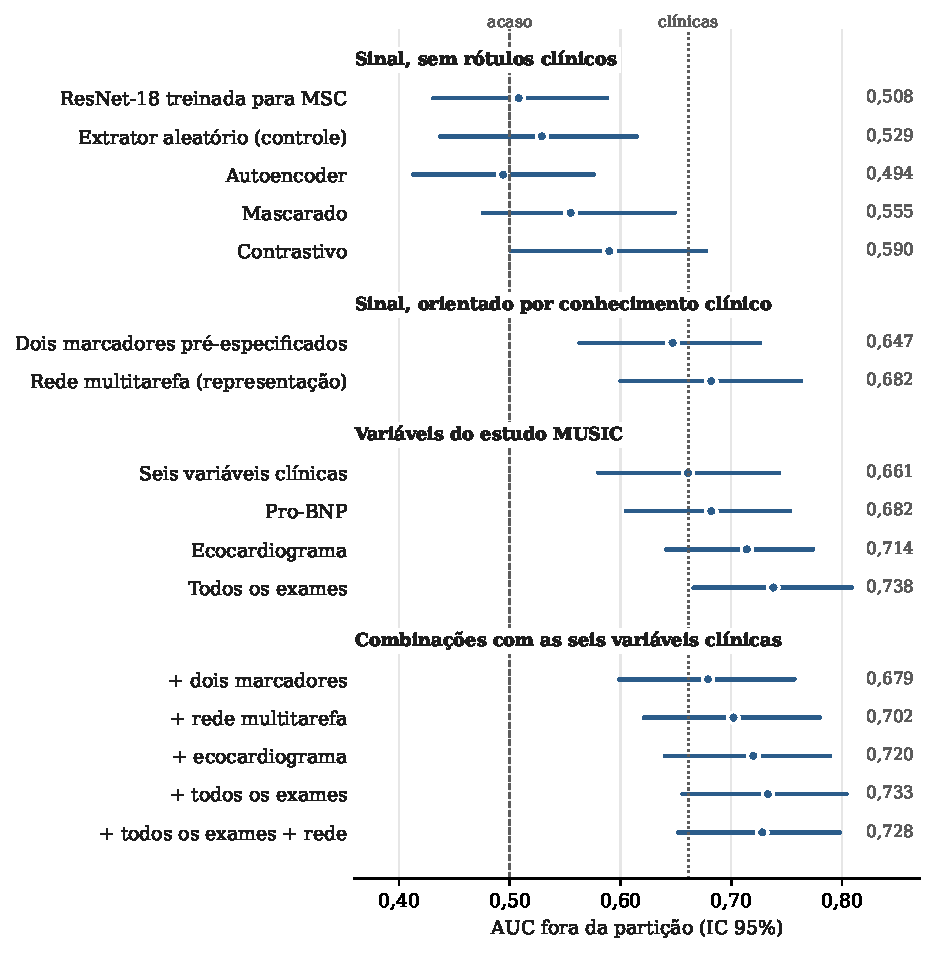
\includegraphics[width=15cm]{figuras/resultados_rotulos_substitutos.pdf}
	}{
		\Fonte{elaborado pelo autor (2026). Linha tracejada: acaso; linha
			pontilhada: seis variáveis clínicas.}
	}
\end{figure}

\subsection{Marcadores pré-especificados}
\label{subsec:res-pre-especificados}

Os dois marcadores pré-especificados --- variação da frequência cardíaca
média ao longo do dia e carga de ectopia --- alcançaram, sozinhos, \gls{AUC}
entre 0,635 e 0,660 conforme a derivação, próximas das seis variáveis
clínicas. Com elas, a \gls{AUC} ficou entre 0,679 e 0,683 nas quatro versões
(derivações X, Y e Z e a derivação de melhor qualidade), com ganho de 0,014 a
0,017 sobre as variáveis clínicas, não significativo. Os casos apresentaram
menor variação da frequência ao longo do dia (desvio-padrão de 7,0 contra
8,5\,bpm) e maior carga de ectopia. Quando todos os marcadores foram usados com
seleção L1, o desempenho caiu à medida que o número de colunas cresceu: de
0,68 com 8 a 10 colunas para 0,57 com 138, efeito do sobreajuste com 33 casos
de treinamento.

\subsection{Rede multitarefa}
\label{subsec:res-multitarefa}

A rede aprendeu parte dos atributos a partir de janelas de 30~segundos. Nos
pacientes de teste, distinguiu QRS acima de 120\,ms com \gls{AUC} de 0,92,
\gls{TVNS} com 0,81, ondas Q com 0,78 e hipertrofia ventricular com 0,74, e
explicou 59\,\% da variância da duração do QRS e 20\,\% da \gls{FEVE}. Não
aprendeu a classe \gls{NYHA}, o tamanho do átrio esquerdo nem as medidas do
ventrículo direito.

Sem nenhuma variável clínica, a representação aprendida alcançou \gls{AUC} de
0,682, equivalente à das seis variáveis clínicas
(\autoref{tab:res-substitutos}). Uma ResNet-18 treinada diretamente
para a morte súbita havia obtido 0,508
(\autoref{sec:res-redes}). Com as variáveis clínicas, a representação
chegou a 0,702, valor igual ao das variáveis clínicas acrescidas da
\gls{FEVE} e do Pro-BNP medidos (0,705). Quando todos os exames medidos já
estavam no modelo, a representação não acrescentou informação: diferença de
$-0{,}005$ [$-0{,}042$; $+0{,}029$], $p = 0{,}75$. Os valores previstos dos
atributos tiveram desempenho inferior ao da representação (0,646 com as
variáveis clínicas).

\begin{table}[h!]
	\captionsetup{width=15cm}
	\Caption{\label{tab:res-substitutos} Desempenho dos modelos com
		representações aprendidas e com os exames do estudo}
	\IBGEtab{}{
		\begin{tabular}{lccc}
			\toprule
			Modelo                                  & \gls{AUC} [\gls{IC} 95\,\%] & Sensib. & Especif. \\
			\midrule \midrule
			Seis variáveis clínicas                 & 0,661 [0,580--0,743] & 0,58 & 0,67 \\
			\midrule
			Rede multitarefa                        & 0,682 [0,600--0,763] & 0,51 & 0,80 \\
			Rede multitarefa + clínicas             & 0,702 [0,621--0,780] & 0,55 & 0,74 \\
			Valores previstos + clínicas            & 0,646 [0,557--0,726] & 0,49 & 0,72 \\
			Contrastivo                             & 0,590 [0,501--0,677] & 0,64 & 0,45 \\
			Contrastivo + clínicas                  & 0,634 [0,551--0,727] & 0,64 & 0,57 \\
			\midrule
			Clínicas + \gls{FEVE} + Pro-BNP         & 0,705 [0,617--0,780] & 0,64 & 0,68 \\
			Clínicas + ecocardiograma               & 0,720 [0,640--0,789] & 0,65 & 0,64 \\
			Clínicas + todos os exames              & 0,733 [0,656--0,804] & 0,71 & 0,64 \\
			Clínicas + todos os exames + rede       & 0,728 [0,652--0,798] & 0,73 & 0,64 \\
			\bottomrule
		\end{tabular}
	}{
		\Fonte{elaborado pelo autor (2026). Limiar de Youden escolhido por
			validação cruzada interna ao treinamento de cada partição.
			Prevalência de morte súbita: 10,6\,\%.}
	}
\end{table}

\subsection{Aprendizado autossupervisionado}
\label{subsec:res-autossupervisionado}

Sem rótulos, os padrões encontrados foram fracos. O método contrastivo
aprendeu a reconhecer janelas do mesmo paciente, com queda contínua da perda
de validação, e superou o extrator aleatório (0,590 contra 0,529), mas ficou
abaixo da rede multitarefa. No autoencoder e no método mascarado, a perda de
reconstrução permaneceu praticamente constante desde a primeira época, e o
desempenho (0,494 e 0,555) ficou no nível do extrator aleatório. Com as
variáveis clínicas, nenhum dos três diferiu delas.

\subsection{Variáveis do estudo e atributos aprendidos}
\label{subsec:res-variaveis}

Entre os exames do estudo, o ecocardiograma foi o grupo mais informativo:
sozinho, alcançou \gls{AUC} de 0,714 e, somado às variáveis clínicas, 0,720
(diferença de $+0{,}058$, $p = 0{,}072$). O Pro-BNP acrescentou $+0{,}047$
($p = 0{,}054$), enquanto o \gls{ECG} de repouso ($+0{,}022$) e os resumos do
Holter ($+0{,}012$) pouco acrescentaram. O conjunto de todos os exames,
sem as variáveis clínicas, alcançou 0,738.

A \autoref{tab:res-variaveis} compara, para cada atributo, sua capacidade de
discriminar a morte súbita e o quanto a rede o aprendeu. Os atributos mais
associados ao desfecho --- tamanho do átrio esquerdo, Pro-BNP, \gls{FEVE} e
diâmetros do ventrículo esquerdo --- foram os menos aprendidos; os mais bem
aprendidos --- QRS largo, hipertrofia, ondas Q --- pouco discriminaram o
desfecho. A ordenação é exploratória, por usar a coorte inteira.

\begin{table}[h!]
	\captionsetup{width=15cm}
	\Caption{\label{tab:res-variaveis} Discriminação da morte súbita por
		atributo isolado e aprendizado do atributo pela rede multitarefa}
	\IBGEtab{}{
		\begin{tabular}{llcc}
			\toprule
			Atributo                                & Exame          & \gls{AUC} para \gls{MSC} & Aprendido pela rede \\
			\midrule \midrule
			Tamanho do átrio esquerdo               & ecocardiograma & 0,701 & $R^2 = 0{,}02$ \\
			Pro-BNP                                 & laboratório    & 0,682 & $R^2 = 0{,}11$ \\
			\gls{FEVE}                              & ecocardiograma & 0,650 & $R^2 = 0{,}20$ \\
			Dupletes ventriculares                  & Holter         & 0,639 & $R^2 = 0{,}28$ \\
			Diâmetro sistólico do VE                & ecocardiograma & 0,631 & $R^2 = 0{,}19$ \\
			Diâmetro diastólico do VE               & ecocardiograma & 0,629 & $R^2 = 0{,}17$ \\
			Extrassístoles ventriculares em 24\,h   & Holter         & 0,620 & $R^2 = 0{,}27$ \\
			\midrule
			Ondas Q                                 & \gls{ECG}      & 0,567 & \gls{AUC} = 0,78 \\
			\gls{TVNS}                              & Holter         & 0,550 & \gls{AUC} = 0,81 \\
			Hipertrofia ventricular esquerda        & \gls{ECG}      & 0,517 & \gls{AUC} = 0,74 \\
			QRS acima de 120\,ms                    & \gls{ECG}      & 0,495 & \gls{AUC} = 0,92 \\
			\bottomrule
		\end{tabular}
	}{
		\Fonte{elaborado pelo autor (2026). \gls{AUC} de regressão logística com
			o atributo isolado, fora da partição; aprendizado medido nos pacientes
			de teste. VE: ventrículo esquerdo.}
	}
\end{table}

\subsection{Síntese}
\label{subsec:res-substitutos-sintese}

Treinada para prever atributos clínicos em vez do desfecho, a rede extraiu
do Holter uma representação com o mesmo poder discriminativo das variáveis
clínicas, sem usar nenhuma delas. Essa representação, porém, corresponde em
grande parte à informação já medida pelos exames: não acrescentou valor
quando eles estavam disponíveis, e os atributos com maior valor prognóstico,
de natureza estrutural, foram justamente os que a rede aprendeu pior. Sem
nenhum rótulo, o aprendizado autossupervisionado não encontrou padrões
comparáveis.


\section{Eletrocardiograma de repouso de alta resolução}
\label{sec:resultados-cnnlstm-repouso}

A seção anterior avaliou arquiteturas distintas sobre a mesma modalidade de
exame. Esta seção altera a modalidade: em lugar do registro
ambulatorial de 24\,horas, emprega-se o eletrocardiograma de repouso de alta
resolução, disponível para parte da coorte e adquirido sob condições
controladas.

A mudança responde a uma hipótese específica. O registro de 24\,horas
contempla o paciente em sono, repouso, esforço e estresse, além de artefatos
de movimento e de deslocamento de eletrodos. Essa variabilidade é alheia ao
desfecho e pode dificultar a identificação de padrões morfológicos. O exame
de repouso, por sua vez, é adquirido com o paciente deitado e imóvel, em
ambiente controlado, e a 1\,000\,Hz --- cinco vezes a frequência de
amostragem do Holter.

\subsection{Dados e arquitetura}
\label{subsec:cnnlstm-dados}

O exame de repouso tem duração aproximada de 20\,minutos e está disponível
para 380 dos 517 pacientes da coorte. A arquitetura adotada processa o exame
integral, e não janelas amostradas: cada paciente corresponde a um único
tensor de $1\,136\,000$ amostras por derivação, descartados 30\,segundos em
cada extremidade. Treze registros mais curtos que esse comprimento foram
excluídos, restando 367 pacientes e 41 eventos --- prevalência de 11,2\,\%.

A arquitetura foi adaptada de \citeonline{freire2025scd}, que a propôs para
estratificação de risco de morte súbita cardíaca por análise de
sobrevivência. Três blocos convolucionais com passo e dilatação reduzem o sinal em
aproximadamente 50\,000 vezes, convertendo $1\,136\,000$ amostras em 21
posições temporais; sobre essa sequência opera uma rede recorrente de memória
longa e curta com duas camadas e 128 unidades ocultas, cujo último estado
alimenta o classificador. A compressão agressiva é o que viabiliza o
processamento do exame integral: arquiteturas convencionais, com redução de
fator quatro por bloco, não comportariam entrada desse comprimento.

O modelo possui $321\,825$ parâmetros treináveis, dos quais cerca de 72\,\%
pertencem à camada recorrente. Em relação à implementação original, três
adaptações foram necessárias: a saída passou a fornecer um valor escalar por
paciente, compatível com a função de perda de entropia cruzada binária; a
camada densa destinada a variáveis tabulares, presente na versão original
ainda quando não utilizada, foi suprimida; e acrescentou-se verificação do
comprimento mínimo da entrada, uma vez que a compressão de aproximadamente
50\,000 vezes inviabiliza sinais mais curtos que o previsto. A validação cruzada empregou cinco partições,
com 219 ou 220 pacientes no treinamento, 74 na validação interna e 73 ou 74
no conjunto de teste.

\subsection{Desempenho}
\label{subsec:cnnlstm-desempenho}

A \gls{AUC} sobre as predições fora da amostra foi de 0,514, com intervalo de
confiança de 95\,\% entre 0,425 e 0,610. O intervalo contém o valor 0,5. Os
resultados por partição constam da \autoref{tab:cnnlstm-folds}.

% ---- TABELA 1: desempenho por partição ----
\begin{table}[h!]
	\captionsetup{width=13cm}
	\Caption{\label{tab:cnnlstm-folds} Desempenho da arquitetura CNN-LSTM
		sobre o exame de repouso, por partição}
	\IBGEtab{}{
		\begin{tabular}{crrrrr}
			\toprule
			Partição                          & \multicolumn{1}{c}{AUC}            & \multicolumn{1}{c}{AP} &
			\multicolumn{1}{c}{Sensibilidade} & \multicolumn{1}{c}{Especificidade} &
			\multicolumn{1}{c}{VPP}                                                                                                 \\
			\midrule \midrule
			0                                 & 0,549                              & 0,164                  & 0,444 & 0,723 & 0,160 \\
			1                                 & 0,648                              & 0,185                  & 0,625 & 0,606 & 0,156 \\
			2                                 & 0,616                              & 0,160                  & 0,375 & 0,708 & 0,125 \\
			3                                 & 0,564                              & 0,158                  & 0,125 & 0,923 & 0,167 \\
			4                                 & 0,555                              & 0,145                  & 0,750 & 0,246 & 0,107 \\
			\midrule
			Média                             & 0,586                              & 0,162                  & 0,464 & 0,641 & 0,151 \\
			Desvio-padrão                     & 0,044                              & 0,015                  & 0,240 & 0,249 & 0,029 \\
			\midrule
			\textit{Out-of-fold}              & 0,514                              & 0,124                  & 0,537 & 0,451 & 0,110 \\
			\bottomrule
		\end{tabular}
	}{
		\Fonte{elaborado pelo autor (2026).}
	}
\end{table}

Chama atenção a discrepância entre as duas estimativas de \gls{AUC}: a média
entre partições, de $0{,}586 \pm 0{,}044$, supera em 0,072 a estimativa
agrupada de 0,514. Trata-se da maior diferença observada entre todos os
experimentos realizados.

A explicação reside na calibração. Cada partição ajusta um modelo
independente, e as probabilidades produzidas situam-se em escalas distintas.
Dentro de uma partição, o ordenamento relativo dos pacientes é razoável ---
donde os valores entre 0,549 e 0,648. Ao reunir as predições das cinco
partições em um ordenamento único, as escalas não coincidem, e um paciente de
baixo risco segundo um modelo pode receber probabilidade superior à de um
paciente de alto risco segundo outro. A estimativa agrupada, embora inferior,
é a que reflete o desempenho esperado em aplicação, na qual um único modelo
ordenaria todos os pacientes.

A \gls{AP} agrupada, de 0,124, supera marginalmente a prevalência de 0,112.

\subsection{Comparação entre modalidades}
\label{subsec:cnnlstm-comparacao}

A \autoref{tab:comparacao-modalidades} confronta os resultados obtidos nas
duas modalidades de exame.

% ---- TABELA 2: comparação entre modalidades ----
\begin{table}[h!]
	\captionsetup{width=15cm}
	\Caption{\label{tab:comparacao-modalidades} Comparação entre as
		modalidades de exame avaliadas}
	\IBGEtab{}{
		\begin{tabular}{llrrr}
			\toprule
			Modalidade              & Arquitetura                 & \multicolumn{1}{c}{$n$ / eventos} &
			\multicolumn{1}{c}{AUC} & \multicolumn{1}{c}{IC 95\%}                                                            \\
			\midrule \midrule
			Holter 24\,h            & CNN mínima                  & 517 / 55                          & 0,523 & 0,440--0,612 \\
			Holter 24\,h            & ResNet-18 reduzida          & 517 / 55                          & 0,504 & 0,420--0,588 \\
			Holter 24\,h            & ResNet-18 completa          & 517 / 55                          & 0,508 & 0,431--0,588 \\
			Holter 24\,h            & ResNet-18 com atenção       & 517 / 55                          & 0,493 & 0,419--0,577 \\
			Repouso 20\,min         & CNN-LSTM                    & 367 / 41                          & 0,514 & 0,425--0,610 \\
			\bottomrule
		\end{tabular}
	}{
		\Fonte{elaborado pelo autor (2026).}
	}
\end{table}

O valor obtido sobre o exame de repouso fica dentro da faixa observada com o
Holter: as diferenças em relação às redes da tabela vão de $-0{,}009$ a
$+0{,}021$, inferiores a um décimo da amplitude dos intervalos de confiança,
que se sobrepõem integralmente. Não há, portanto, evidência de superioridade de uma
modalidade sobre a outra.

Duas ressalvas restringem ainda mais a comparação. A primeira é que as
coortes diferem: 367 pacientes com 41 eventos no exame de repouso, contra 517
com 55 no Holter. Parte de qualquer diferença observada pode decorrer da
composição da amostra, e não da modalidade. A comparação rigorosa exigiria
avaliar ambas as modalidades sobre o mesmo subconjunto de pacientes.

A segunda é que a arquitetura também difere. O exame de repouso foi avaliado
com a CNN-LSTM, enquanto o Holter o foi com arquiteturas convolucionais e
residuais. O experimento altera simultaneamente duas variáveis, o que impede
atribuir eventual diferença a qualquer uma delas isoladamente.

\subsection{Matriz de confusão}
\label{subsec:cnnlstm-confusao}

% ---- TABELA 3: matriz de confusão ----
\begin{table}[h!]
	\captionsetup{width=11cm}
	\Caption{\label{tab:cnnlstm-confusao} Matriz de confusão agregada da
		arquitetura CNN-LSTM sobre o exame de repouso}
	\IBGEtab{}{
		\begin{tabular}{lrr}
			\toprule
			                               & \multicolumn{1}{c}{Predito: sobrevivente} &
			\multicolumn{1}{c}{Predito: óbito}                                               \\
			\midrule \midrule
			Sobrevivente ($n = 326$)       & 147                                       & 179 \\
			Óbito por \gls{MSC} ($n = 41$) & 19                                        & 22  \\
			\bottomrule
		\end{tabular}
	}{
		\Fonte{elaborado pelo autor (2026).}
	}
\end{table}

Dos 41 óbitos por morte súbita cardíaca, 22 foram identificados ---
sensibilidade de 0,537 --- com 179 falsos positivos entre os 326
sobreviventes. O \gls{VPP} de 0,110 permanece praticamente igual à
prevalência de 0,112.

\subsection{Síntese}
\label{subsec:cnnlstm-sintese}

A hipótese que motivou o experimento --- de que a menor presença de
artefatos no exame de repouso favoreceria a identificação de padrões
morfológicos --- não se confirmou. O desempenho permaneceu na mesma faixa
observada com o Holter, com intervalo de confiança compatível com o acaso.

O resultado acrescenta elemento relevante ao conjunto de evidências: a
limitação observada não decorre da qualidade do sinal nem da presença de
artefatos de movimento, uma vez que persiste em registros adquiridos sob
condições controladas e com frequência de amostragem cinco vezes superior.
